\documentclass[9pt]{beamer}
% \documentclass[notes, handout, 9pt]{beamer}
% \documentclass[handout, 9pt]{beamer}

\usepackage{import}
\subimport{../}{preamble.tex}
\subimport{../}{beamer-theme.tex}
\usepackage{svg}

% Location for all figures / pictures
\graphicspath{{pictures/}{figures/}}

% % Figures inline
\usepackage{tikz}
\usepackage{pgfplots}
\usetikzlibrary{calc}
\usetikzlibrary{shapes.multipart}
\usetikzlibrary{decorations.pathreplacing}
\usetikzlibrary{arrows.meta}
\usepgfplotslibrary{fillbetween}

%--------------------------------------------------
% Presentation Information
%--------------------------------------------------
\title[Continuous Optimization]{Performance Estimation Programming}
\author[]{\textbf{Bart Van Parys}}
\date[]{Fall 2026}
%--------------------------------------------------

\begin{document}

\begin{frame}

  \maketitle

  \vspace{-2em}

    \begin{center}
    \begin{tabular}{lll}
      Instructor : & \textbf{Bart Van Parys} & \textbf{(\href{mailto:mastermath@vanparys.xyz}{mastermath@vanparys.xyz})} \\
    \end{tabular}
  \end{center}

\end{frame}

\begin{frame}[label=averaging]{Nonsmooth Convex Optimization}

  \begin{center}
  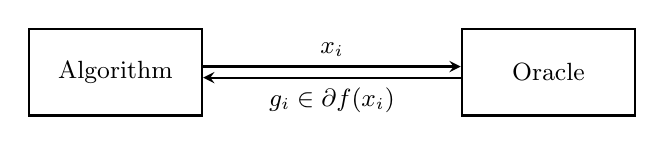
\begin{tikzpicture}[
      box/.style={draw, thick, minimum width=2.2cm, minimum height=1.1cm,
                  align=center, font=\small},
      >=stealth, thick,
    ]
    \node[box] (alg) at (0,0) {Algorithm};
    \node[box] (ora) at (5.5,0) {Oracle};

    % query: Algorithm -> Oracle (above)
    \draw[->] ([yshift=2pt]alg.east) -- ([yshift=2pt]ora.west)
      node[midway, above, font=\small] {$x_i$};
    % answer: Oracle -> Algorithm (below)
    \draw[->] ([yshift=-2pt]ora.west) -- ([yshift=-2pt]alg.east)
      node[midway, below, font=\small] {$g_i \in \partial f(x_i)$};
\end{tikzpicture}
  \end{center}

  \vfill

  \textbf{Subgradient Descent:}
  \begin{align*}
    x_{i+1} = & x_i - h_i g_i \quad \forall i \in [0, \dots, N-1]\\                                     
    x_{A} = & \textstyle \tfrac{\sum_{i=0}^N h_i x_i}{\sum_{i=0}^N h_i.}
  \end{align*}
  
  \vfill  
  Lecture 8:
  \[
    f(x_{A}) - f(x_\star) \leq E(h) = \textstyle\tfrac{(R^2 + L^2\sum_{i=0}^N h_i^2)}{(2\sum_{i=0}^N h_i)}
  \]
  so that with \textit{constant} stepsize $h_i = R/(L\sqrt{N+1})$ we have $$\min_{h_0\geq 0, \dots, h_{N}\geq 0} E(h) = \frac{RL}{\sqrt{N+1}}.$$
  
\end{frame}

\begin{frame}[label=textbook]{Subgradient Method Textbook Analysis (see Lecture 8)}

  Shorthand: $f_i \defn f(x_i)$ and $g_i \in \partial f(x_i)$ for $i \in \{0, \dots, N, A, \star\}$.

  \begin{itemize}
  \item<1-> The iterates $x_i$ for $i\in [0, \dots, N]$ satisfy the recursion
    \[
      \blue{\norm{ x_{i+1}-x_\star}^2\leq \norm{x_i-x_\star}^2 - 2 h_i \langle  g_i , x_i -x_\star \rangle + h_i^2 \norm{g_i}^2} .
    \]
  \item<2-> The subgradient inequality between $x_i$ and $x_\star$ ensures $\red{\langle  g_i, x_\star-x_i\rangle \leq f_\star-f_i}$ for all $i\in [0, \dots, N]$. Hence,
    \[
      2 h_i (f_i-f_\star) \leq \norm{x_i-x_\star}^2_2 - \norm{x_{i+1}-x_\star}^2 + h_i^2 \norm{ g_i}^2.
    \]
  \item<3-> Telescopic sum over $i\in [0, \dots, N]$ gives
    \[
      \sum_{i=0}^N 2 h_i (f_i-f_\star) \leq \norm{x_0-x_\star}_2^2 - \norm{x_{N+1}-x_\star}_2^2 + {\sum_{i=0}^N h_i^2 \norm{ g_i}^2}.
    \]
  \item<4-> The subgradient inequality between $x_i$ and $\blue{x_A= \sum_{i=0}^N h_i x_i/\sum_{i=0}^N h_i}$ ensures $\red{\langle g_A, x_i-x_A\rangle \leq f_i-f_A}$.
  \item<4-> As $\red{\norm{ g_i}^2\leq L^2}$ and $\color{green}{\norm{x_0-x_\star}^2\leq R^2}$, we get by multiplying by $h_i/\sum_{i=0}^N h_i$ and summing over $i\in [0,\dots, N]$
    \[
      f_A - f_\star\leq \frac{\sum_{i=0}^N h_i (f_i-f_\star)}{\sum_{i=0}^N h_i} \leq \frac{R^2+{L^2 \sum_{i=0}^N h_i^2}}{2 \sum_{i=0}^N h_i}.
    \]
  \end{itemize}

  
\end{frame}

\begin{frame}{Adversarial Perspective}

  \emph{Resisting} the proof analysis is then an optimization problem over this finite data:

    \begin{equation*}
      \begin{array}{rl}
        \max &  f_A-f_\star\\[0.5em]
        \st  & f_i \defn f(x_i), ~g_i \in \partial f(x_i) \quad \forall i \in \{0, \dots, N+1, A, \star\} \\[0.5em]
             & \blue{\norm{ x_{i+1}-x_\star}^2\leq \norm{x_i-x_\star}^2 - 2 h_i \langle g_i , x_i -x_\star \rangle + h_i^2 \norm{g_i}^2} \\[0.5em]
                    & \blue{x_A= \sum_{i=0}^N h_i x_i/\sum_{i=0}^N h_i}\\[0.5em]
                                     & \color{green}{\norm{x_0-x_\star}^2\leq R^2},\\[0.5em]
                                     & \red{\langle  g_i, x_\star-x_i\rangle \leq f_\star-f_i} \quad \forall i\in [0, \dots, N], \\[0.5em]
                                                & \red{\langle g_A, x_i-x_A\rangle \leq f_i-f_A} \quad \forall i\in [0, \dots, N],\\[0.5em]
                   & \red{\norm{ g_i}^2\leq L^2} \quad \forall i\in [0, \dots, N]\\[0.5em]
      \end{array}
    \end{equation*}
    a nonconvex problem.

\end{frame}

\begin{frame}{Linearization: a Gram Matrix}

  The objective and every constraint depend on the iterates only through
  \emph{pairwise inner products}!
  \vfill
  Let
  \[
    P = \big[\, x_0, \dots, x_{N+1}, x_A, x_\star, ~ g_0, \dots, g_N, g_A \,\big] \in \Re^{d \times m},
  \]
  and collect all their inner products in the \emph{Gram matrix}
  \[
    G = P^\top P \in \mathbb{S}_+^m.
  \]

  \vfill

  Every ingredient is then \emph{linear} in $G$ (and in $F = (f_i)$), e.g.,
  \begin{align*}
    \norm{x_i - x_\star}^2 &= G_{x_i, x_i} - 2\, G_{x_i, x_\star} + G_{x_\star, x_\star}, \\
    \langle g_i, x_i - x_\star \rangle &= G_{g_i, x_i} - G_{g_i, x_\star}, \\
    \norm{g_i}^2 &= G_{g_i, g_i}.
  \end{align*}

  \vfill

  The bilinear (nonconvex) terms become \emph{linear} entries of $G$. Conversely,
  whenever $G \succeq 0$ we can factor $G = P^\top P$ and read off the worst-case iterates
  and subgradients.

\end{frame}

\begin{frame}{Demo}

\end{frame}

\end{document}
%%% Local Variables:
%%% mode: latex
%%% TeX-master: t
%%% End:
